\documentclass{mcmthesis}
\mcmsetup{CTeX = false,   % 使用 CTeX 套装时,设置为 true
        tcn = 2013647, problem = D,
        sheet = true, titleinsheet = true, keywordsinsheet = true,
        titlepage = false, abstract = true}
    
\usepackage{palatino}
\usepackage{lipsum}
\usepackage{fancyhdr}
\usepackage{extramarks}
\usepackage{amsmath}
\usepackage{amsthm}
\usepackage{amsfonts}
\usepackage{tikz}
\usepackage[plain]{algorithm}
\usepackage{algpseudocode}
\usepackage{arydshln}
\usepackage{mathtools}
\usepackage{cases}
\usepackage{listings}
%\usepackage[numbered]{mcode}
\usepackage{booktabs}
\usepackage{graphicx}
\usepackage{subfigure}
\usepackage{indentfirst}
\usepackage{pythonhighlight}
\usepackage{url}

\newcommand{\upcite}[1]{\textsuperscript{\textsuperscript{\cite{#1}}}}

\title{Team Evaluation Using Network Science and Classifier}
\date{\today}
\begin{document}
    \begin{abstract}

		In order to provide effective team cooperation mode and strategies for Huskies’ soccer coach for future improvement, we built passing networks combined with machine learning models based on comprehensive analysis on the data given.
		
		For task 1, we firstly did preliminary analysis on the correlation of the location of passing the ball and the outcome of the match. The results turned out that there was little correlation between the two. Hence, secondly, we created the networks from multiple-scales analysis. We computed different network metrics, which represented different meanings of centrality, and tried to find correlation between these metrics and the outcome of the match. 
		
		For task 2, we created the Activity Level Frequency Model based on the network analysis, which could represent the frequency a team made of certain actions in one match. In addition, we did Fourier transformation to this model to calculate how many effective actions a team made in one match. Further, we utilized machine learning techniques to fit our models on the data. By evaluating our machine learning models, we evaluated how accurate our metrics describe a soccer team.
		
		For task 3, we summarized the prediction results using our models, based on which, we offered specific suggestions to Huskies coach for promoting the team's performance next season.
		
		For task 4, based on the analysis of the Huskies team, we extended the setting of teamwork to complex social backgrounds, and proposed the understanding of Group Dynamics, how to design a high-quality team, and additional significant indicators that affect teamwork.


\begin{keywords}
Network Science; Network Metrics; Team Evaluation; Random Forest; Fourier Transformation; Group Dynamics
\end{keywords}
\end{abstract}
\maketitle
%% Generate the Table of Contents, if it's needed.
%% \tableofcontents
%% \newpage
%%
%% Generate the Memorandum, if it's needed.
%% \memoto{\LaTeX{}studio}
%% \memofrom{Liam Huang}
%% \memosubject{Happy \TeX{}ing!}
%% \memodate{\today}
%% \logo{\LARGE I'm pretending to be a LOGO!}
%% \begin{memo}[Memorandum]
%%   \lipsum[1-3]
%% \end{memo}
%%
\tableofcontents
\setlength{\parindent}{2em}

\newpage

\section{Introduction}

	\subsection{Background}
	With the increasing demand of people in today's society to rely on teamwork to solve increasingly complex social problems in all aspects, our pursuit and exploration of the factors that contribute to team success have become significant and indispensable. People are dedicated to continuous research on optimizing strategies for achieving higher level of teamwork, and competitive team sports is one of the biggest areas that could benefit from these studies. 

	How can we give full play to our team's initiative and break the opponent team’s strategy to win under the strict rules of the game? In order to solve this problem, we not only need to analyze the skill levels and kicking modes of individual players, tactical strategy and internal cooperation of the whole team, individual player's different influence on the team are also important. It is worth noting that the above analysis needs to be carried out under various settings, including own team, opponent teams, different games, different zooms in the playing field and different time periods of the game, so as to achieve a comprehensive, detailed and accurate team analysis and improvement effect.

	\subsection{Restatement of the Problem}
	According to the Huskies coach’s requests, we need to use Huskies’ game data in last season to quantify and regularize the team's structure and dynamic characteristics. Specifically, analyzing how the complex interaction between the players on the field affects the team's scoring, the team's game state and vitality, and puts forward specific improvement suggestions on teamwork for the training and games of Huskies next season based on the analysis.
	
	For Task 1, firstly, we are supposed to build passing networks for the ball passing between players, with players being nodes and passes being links, and then process, model and analyze the passing process of each game to identify network patterns. Secondly, 
	
	For Task 2, determine the specific indicators that affect the quality of teamwork, and build a model from the team level through the combination of these indicators to reflect the structural, configurational, and dynamical aspects of teamwork.
	
	For Task 3, based on the analysis of our team network and model, point out the effective team cooperation mode and strategies for Huskies, and specifically suggest the aspects that they need to improve in the next season.
	
	For Task 4, reflect on our analysis on Huskies, considering the indicators and factors that improve team performance, we are supposed to generalize how to design and build a higher-quality team and point out additional team cooperation indicators needed to analyze a team.
	
	\subsection{Overview of Our Work}
		We firstly did basic analysis on the data given and calculated the correlation with the output. Secondly, we used graph-tool which is a library in C++ to create the network for each match. After that, we computed different network metrics and their correlation with the outcome and the score for each match. Then we created the Activity Level Frequency Model, finding significant results from multiple scales and visualizing the data in a better way. Next, we used some methods of machine learning such as using classifiers like random forest to get the inner visualization of the network metrics and the outcome of the matches. 
		

\section{Analysis of the Problem}
	\subsection{Correlation Analysis and Heat Map}
		According to the data given, we computed the correlation among the passing position, event type, event sub type and the outcome. Here we use the $\phi$ coefficient of chi-squares test, where $\phi=\sqrt{\frac{\mathcal{X}^2}{n}}$. The advantage of using $\phi$ coefficient is it can test the association between several variables and is always bigger than zero. The following is the result. 
		\begin{figure}[h!]
			\centering
			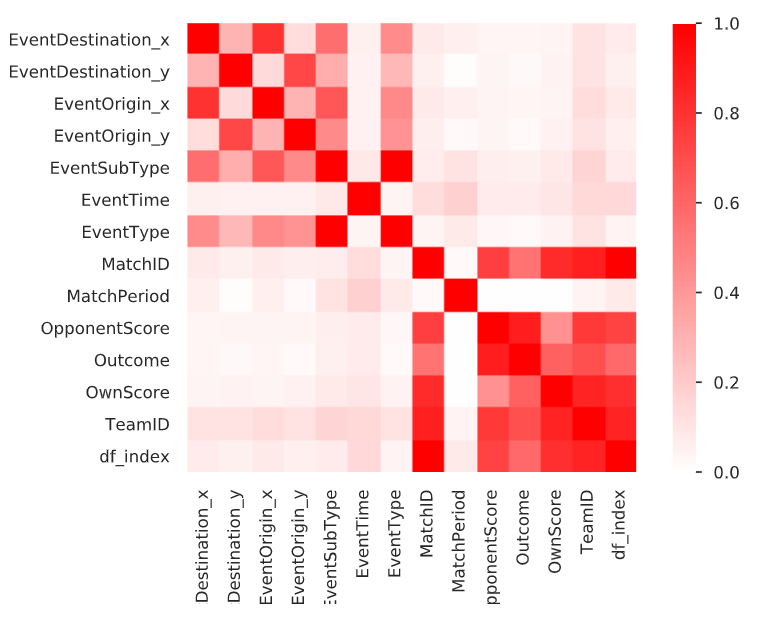
\includegraphics[scale=0.6]{images/cor_1.PNG}
			\caption{$\phi_k$ coefficient between different variables. }
		\end{figure} \\
		
		We can see that the area of passing position and outcome has very weak association. 
		
		
	\subsection{Network Creation}
			We create nodes to represent each player, and add edges between two nodes to represent that they passed one ball. Then we created the network as the following: 
			\begin{figure}[h!]
				\centering
				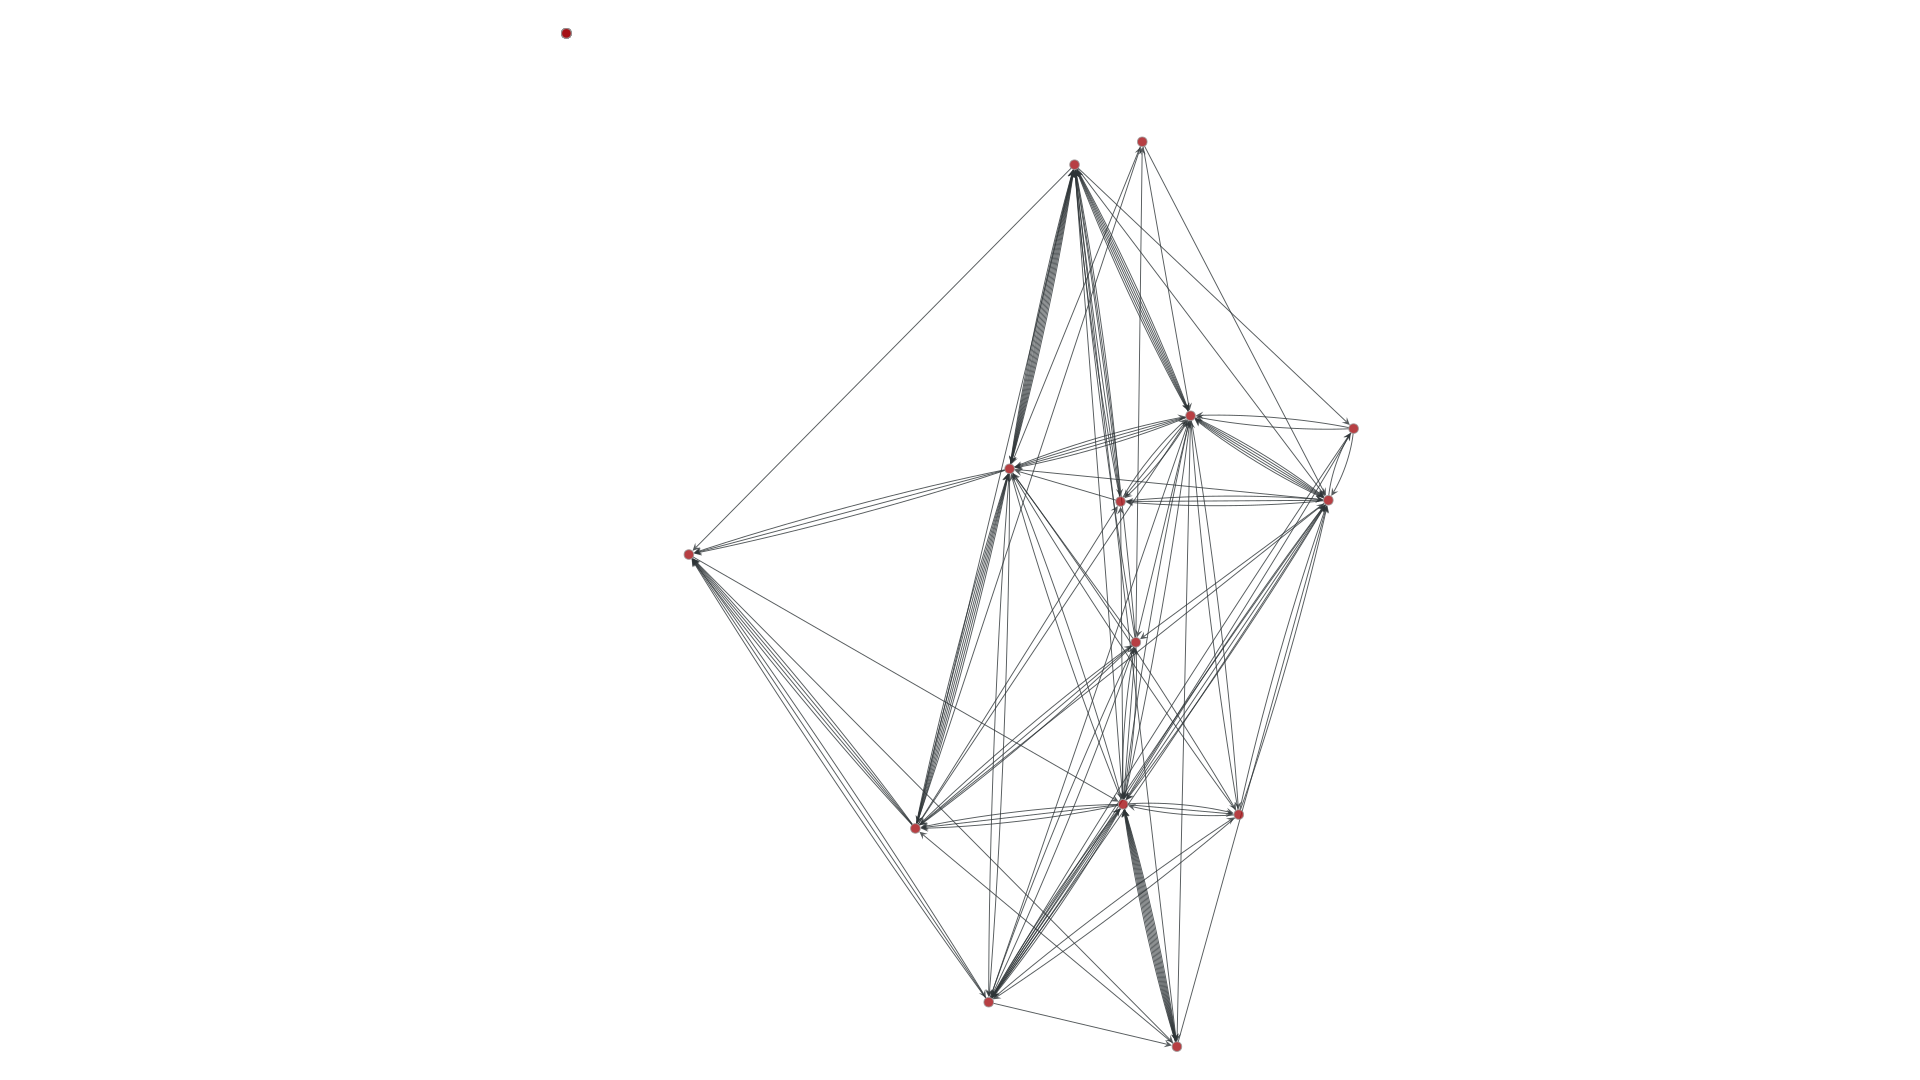
\includegraphics[scale=0.2]{images/network_12.png}
				\caption{Network example plot of the $12^\mathrm{th}$ match. }
			\end{figure} \\
			The thickness of the edges represents the number of passes between two nodes. 
	\subsection{Network Analysis}\label{network-analysis}
		We calculated different metrics to find the correlation with the outcome. 
		\begin{enumerate}
			\item Local Clustering Coefficient\upcite{4} \\
			Our network is a directed graph, here the local clustering coefficient is defined by: 
			$$C_i=\frac{\left|\left\{e_{jk}:v_j,v_k\in N_i,e_{jk}\in E\right\}\right|}{k_i\left(k_i-1\right)}$$
			Where $N_i$ represents the set of the neighbourhoods of vertex $i$, $E$ represents the set of all the edges in this network, $k_i$ represents the number of the neighbourhoods of vertex $i$. Then we calculate the mean value, standard deviation of $C_i$, $i\in \left[0, n\right]$, and get the correlation as the following: 
			\begin{table}[h!]
				\centering
				\begin{tabular}{cccccc}
					\toprule
					 & mean & std & Outcome & OwnScore & ScoreDiff \\
					mean & 1.000000 & 0.631727 & 0.185350 & 0.229202 & -0.103709 \\
					std & 0.631727 & 1.000000 & -0.005841 & 0.189648 & -0.266331 \\
					Outcome & 0.185350 & -0.005841 & 1.000000 & 0.695860 & 0.180965 \\
					OwnScore & 0.229202 & 0.189648 & 0.695860 & 1.000000 & -0.580393 \\
					ScoreDiff & -0.103709 & -0.266331 & 0.180965 & -0.580393 & 1.000000 \\
					\bottomrule
				\end{tabular}
				\caption{Result of correlation of clustering coefficient. }
			\end{table}
			
			\item Closeness Centrality\upcite{4} \\
			Here the closeness centrality can be defined by: 
			$$c_i=\frac{1}{\sum\limits_jd_{ij}}$$
			This metric can represent how tight a network is. The analysis of correlation is as the following: 
			\begin{table}[h!]
				\centering
				\begin{tabular}{cccccc}
					\toprule
					 & mean & std & Outcome & OwnScore & ScoreDiff \\
					mean & 1.000000 & 0.066782 & -0.001622 & 0.102358 & -0.146188 \\
					std & 0.066782 & 1.000000 & 0.107140 & 0.044999 & 0.058649 \\
					Outcome & -0.001622 & 0.107140 & 1.000000 & 0.695860 & 0.180965 \\
					OwnScore & 0.102358 & 0.044999 & 0.695860 & 1.000000 & -0.580393 \\
					ScoreDiff & -0.146188 & 0.058649 & 0.180965 & -0.580393 & 1.000000 \\
					\bottomrule
				\end{tabular}
				\caption{Result of correlation of closeness centrality. }
			\end{table} \\
		
			\item Betweeness Centrality\upcite{4} \\
			Here the betweeness centrality can be defined by: \\
			$$C_B\left(v\right)=\sum\limits_{\substack{s\neq v\neq t\in V \\ s\neq v}}\frac{\sigma_{st}\left(v\right)}{\sigma_{st}}$$
			Here $\sigma_{st}$ is the number of shortest paths from $s$ to $t$. $\sigma_{st}\left(v\right)$ represents the number of shortest paths from s to t that pass through a vertex $v$. This mertric can represents organization of midfield formation. The analysis of correlation is as the following: 
			\begin{table}[h!]
				\centering
				\begin{tabular}{ccccccc}
					\toprule
					 & mean & std & cpd & Outcome & OwnScore & ScoreDiff \\
					mean & 1.000000 & 0.489426 & 0.264283 & 0.124010 & -0.092904 & 0.267839 \\
					std & 0.489426 & 1.000000 & 0.882390 & 0.073674 & 0.028949 & 0.043895 \\
					cpd & 0.264283 & 0.882390 & 1.000000 & -0.000588 & 0.028128 & -0.039186 \\
					Outcome & 0.124010 & 0.073674 & -0.000588 & 1.000000 & 0.695860 & 0.180965 \\
					OwnScore & -0.092904 & 0.028949 & 0.028128 & 0.695860 & 1.000000 & -0.580393 \\
					ScoreDiff & 0.267839 & 0.043895 & -0.039186 & 0.180965 & -0.580393 & 1.000000 \\
					\bottomrule
				\end{tabular}
				\caption{Result of correlation of betweeness centrality. }
			\end{table}
			
			\item Eigenvector Centrality\upcite{4} \\
			Here the eigenvector centrality can be defined by: 
			$$Ax=\lambda x$$
			Where $\lambda$ is the largest eigenvalue of adjacency matrix A. Adjacency matrix for directed network is defined by: 
			$$A_{ij}=\begin{cases}
			1 & \text{if} \left(j,i\right)\in E \\
			0 & \text{otherwise} \\
			\end{cases}$$
			$A_{ij}$ corresponds to the directed edge $j\rightarrow i$. The $v^\mathrm{th}$ component of the related eigenvector then gives the relative centrality score of the vertex $v$ in the network. The correlation analysis is as the following: 
			\begin{table}[h!]
				\centering
				\begin{tabular}{ccccc}
					\toprule
					 & eigenvector & Outcome & OwnScore & ScoreDiff \\
					eigenvector & 1.000000 & 0.156880 & 0.195184 & -0.089405 \\
					Outcome & 0.156880 & 1.000000 & 0.695860 & 0.180965 \\
					OwnScore & 0.195184 & 0.695860 & 1.000000 & -0.580393 \\
					ScoreDiff & -0.089405 & 0.180965 & -0.580393 & 1.000000 \\
					\bottomrule
				\end{tabular}
				\caption{Result of correlation of eigenvector centrality. }
			\end{table} \\
		
			\item Katz Centrality\upcite{4} \\
			Here Katz centrality can be defined by: 
			$$\mathbf{x}=\alpha\mathbf{Ax}+\beta$$
			Where $\mathbf{A}$ is the adjacency matrix defined above, and $\beta$ is the personalization vector. Here we assume $\beta=1$. The correlation analysis is as the following: 
			\begin{table}[h!]
				\centering
				\begin{tabular}{cccccc}
					\toprule
					 & mean & std & Outcome & OwnScore & ScoreDiff \\
					mean & 1.000000 & -0.488159 & -0.054294 & -0.220602 & 0.240535 \\
					std & -0.488159 & 1.000000 & 0.189791 & 0.263458 & -0.145584 \\
					Outcome & -0.054294 & 0.189791 & 1.000000 & 0.695860 & 0.180965 \\
					OwnScore & -0.220602 & 0.263458 & 0.695860 & 1.000000 & -0.580393 \\
					ScoreDiff & 0.240535 & -0.145584 & 0.180965 & -0.580393 & 1.000000 \\
					\bottomrule
				\end{tabular}
				\caption{Result of correlation of Katz centrality. }
			\end{table}
		\end{enumerate}
	
\section{Activity Level Frequency Model Analysis}\label{act-lvl-frq}
	\subsection{Model Creation}
	From the analysis given above, we did not find obvious correlation between centrality metrics and the match outcome.
	
	In this model, we define every event happened in the match will contribute to the four parts: attack, defense, collaborate, foul. And each subevent will contribute different weights to these four parts. We cut the whole match into many small time intervals . Let $S\in \mathbb{R}^{m\times 4}$ to denote the final activity level of the team at the end of the match. 
	$$S=\sum\limits_{i=1}^{n}\left(e_i\cdot\sum\limits_{p_i=1}^{q_i}\alpha_i\right)$$

	Where $n$ is the number of time intervals, $q_i$ is the number of events happening in the $i^\mathbf{th}$ time interval, $\alpha_i^\mathbf{T}\in\mathbb{R}^4$ denotes to the different weights one event contribute to attack, defense, collaborate and foul. $e_i\in\mathbb{R}^m$ which $i^\mathbf{th}$ component is 1 and 0 otherwise. 
	
	The four columns of $S$ represent the activity level of the whole team's attack, defense, collaborate, foul respectively. The list of $\alpha_i$ is in the appendix. We get the result as the following: 
	\begin{figure}[h!]
		\centering
		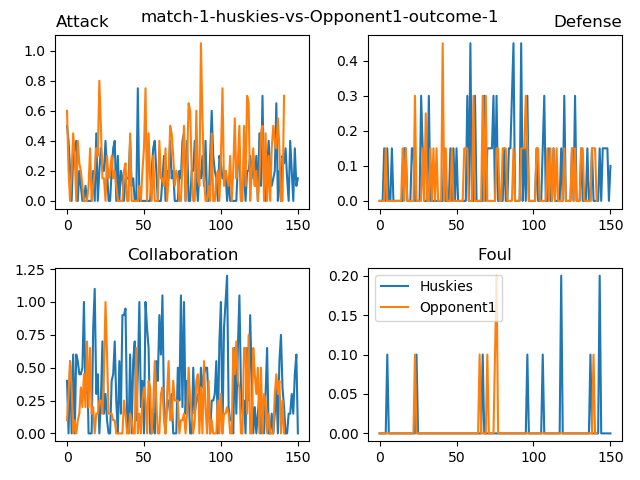
\includegraphics[scale=0.7]{images/match-1-huskies-vs-Opponent1-outcome-1.png}
		\caption{Activity Level of one winning match. }
	\end{figure} \\
	
	We can clearly see that Huskies' collaboration frequency level is larger than Opponent 1. 
	
	\begin{figure}[h!]
		\centering
		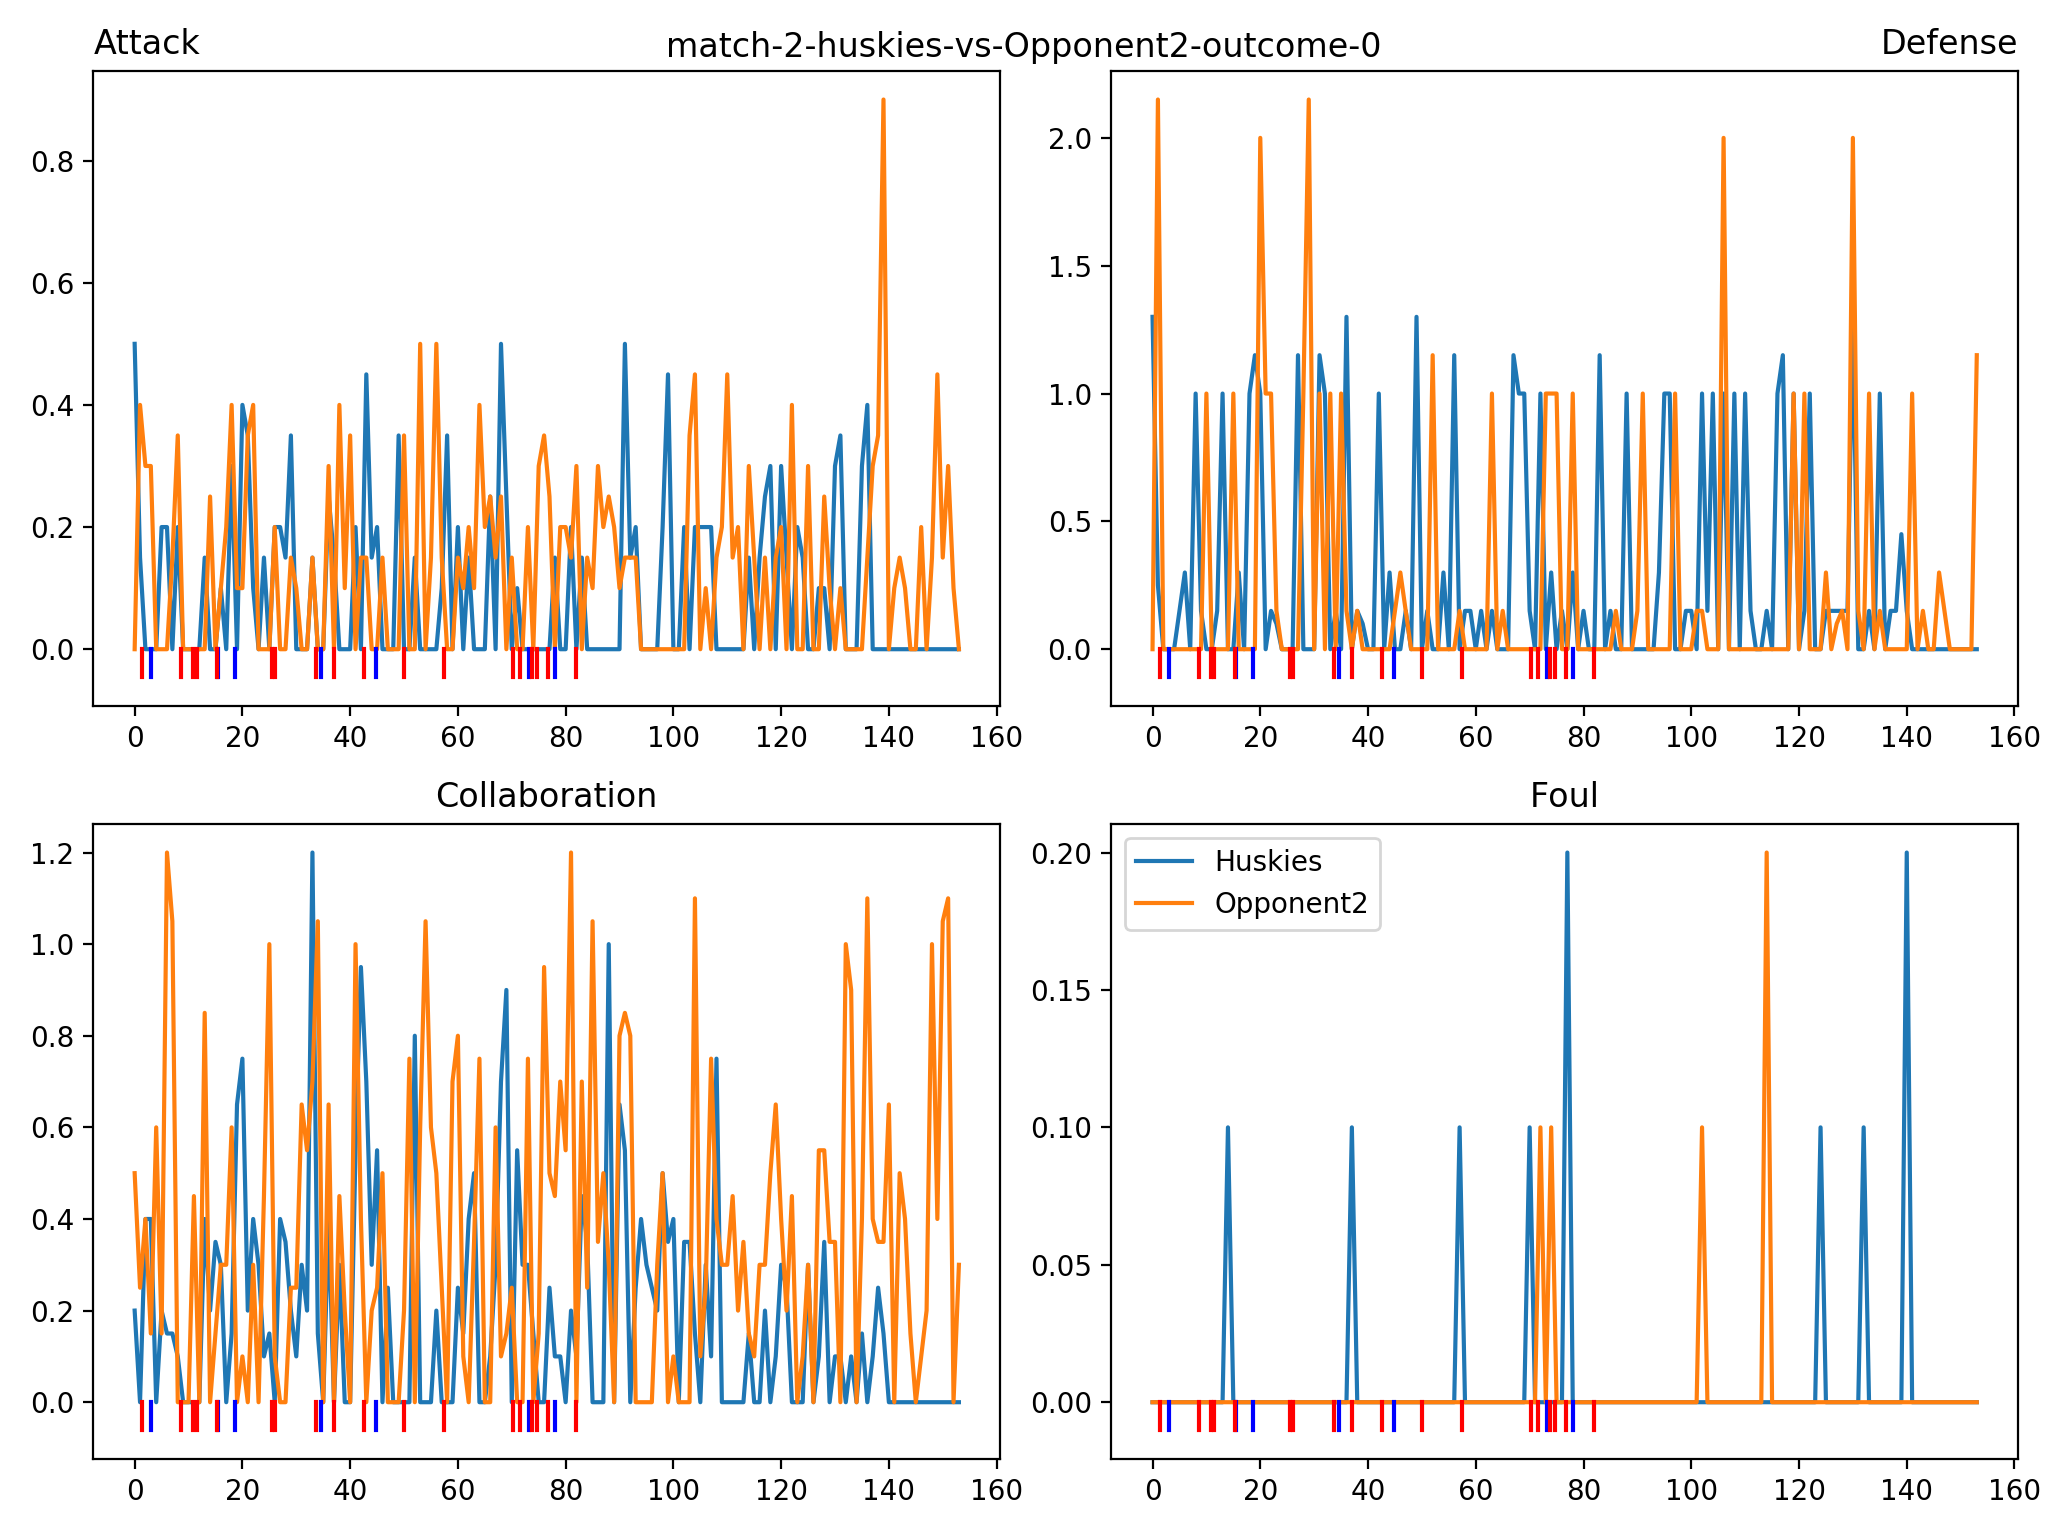
\includegraphics[scale=0.7]{match-2-huskies-vs-Opponent2-outcome-0.png}
		\caption{Activity Level of one tie match. }
	\end{figure}
	
	We can see that although Huskies' collaboration is far worse then Opponent2's, but our defense is really good, so it is a tie match. 
	
	
	\subsection{Fourier Transformation of the Frequency Model}
		Since we've already built the Activity Level Model and got the frequency, it is still not so obvious to find out. So we did Fourier transformation to the activity frequency level model. After the transformation, we can find the response to the high frequency, which means that we can find out how many times one team can attack, defense, collaboration or foul at a certain frequency, the number of effective attacking, collaboration etc. The result is as the following: 
		\begin{figure}[h!]
			\centering
			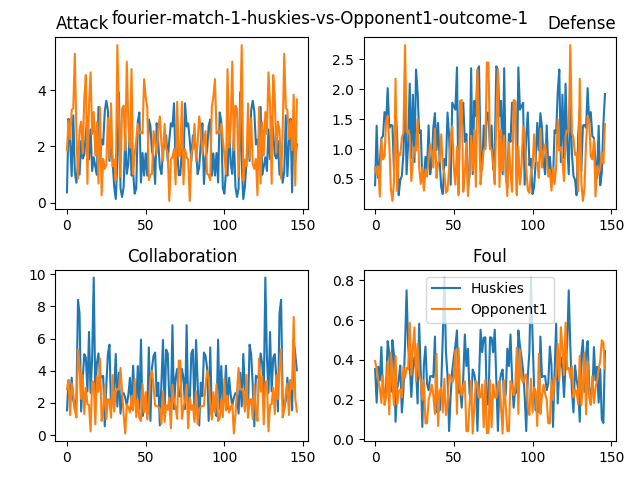
\includegraphics[scale=0.7]{images/fourier-match-1-huskies-vs-Opponent1-outcome-1.png}
			\caption{Fourier Transformation of the first match's frequency model. }
		\end{figure} 
		
		Since the Fourier transformation result is symmetric. So the middle part of each plot represents the response of the highest frequency. Looking at the collaboration part, Huskies' number of high frequency collaboration is much higher than Opponent1. 
		
		Here's one example of a losing match. 
		\begin{figure}[h!]
			\centering
			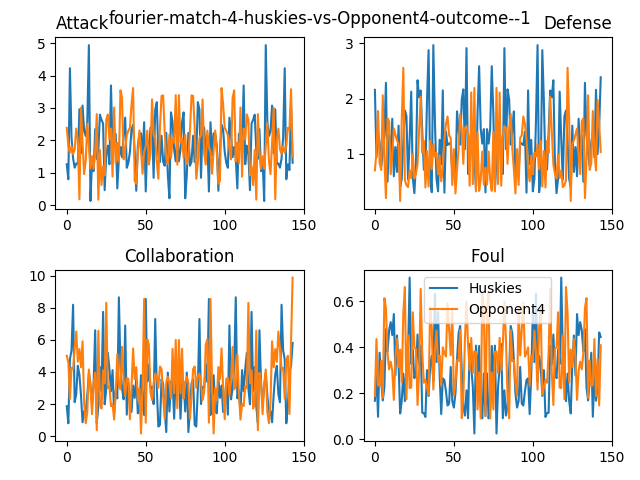
\includegraphics[scale=0.7]{images/fourier-match-4-huskies-vs-Opponent4-outcome--1.png}
			\caption{Fourier Transformation of the $4^\mathrm{th}$ match's frequency model.}
		\end{figure} 
		
		In this figure, we can see that Opponent4's effective collaboration is much higher than Huskies', and their effective attack is also a little bit higher than Huskies'. 


\section{Model Implementations Using Machine Learning}

\subsection{Goals}

Our intended goals to achieve with the help of machine learning techniques are:

\begin{itemize}
    \item generalizing the relationship of some indicators with the overall
    performance of a soccer team\upcite{2}
    \item being able to make prediction of a team's performance in the match
    with the some input indicators
    \item being easy to extended to a more general model that can fit many
    other types of social groups, such as political groups, companies, and nations, as well as being able to provide insights on how to improve their
    performance
\end{itemize}

To be more specific, our model must at least be able to use the network metrics and activity level frequencies introduced above to predict the outcome of a match.

\subsection{Model Selection}

There are plenty of models, widely used in the realm of data science,
to choose from. However, there are several
crucial factors that affects the quality of the final model.

\begin{itemize}
    \item the size of the data
    \item the type of the data (categorical, numerical, etc.)
    \item the evaluation (score) methods
    \item the optimization methods
\end{itemize}

\subsubsection{Data Size}

Since the dataset is very small (extremely small compared to datasets that
many machine learning projects used), it is a good idea to avoid classifiers
that requires a large amount of data in order to manage to reach a satisfying
accuracy. Moreover, the probability of over-fitting appearing is small, 
so regularization is not likely to be needed.

\subsubsection{Data Type}

For data types, we are mainly concerned with the target (output) type, since
the inputs are all numerical data (clustering coefficients, centrality coefficients, etc.) However, we mustn't ignore the fact that some inputs are
matrices while the other are scalar values. We will address this later in this
paper in more details.

In the current context, our output data consists of categorical data (match outcomes). Therefore, classification models are required to make the prediction.

\subsection{Random Forest}

For the classifier model, we chose to use Random Forest to fit the data

\subsubsection{Algorithms}
    The process of the algorithm of random forest is as the following: 
	\begin{enumerate}
		\item Randomly pick a random sample with replacement of the training set, and repeated this process for $m\times n$ times, in order to split into $m$ sub parts, each sub part has $n$ samples, which is same with the number of original training set. This step is called bagging step. 
		\item Created decision trees for each sub set. 
		\item Averaging the predictions from all the individual regression trees.
	\end{enumerate}

\subsubsection{Feature Extraction}

Two sets of feature are extracted in this process, one is the metrics discussed in \ref{network-analysis} Network Analysis and the other one is the metrics introduced in \ref{act-lvl-frq} Activity Level Frequency Model Analysis.

For the network metrics, seven of them are included in the training data, they are Passing Volume, Clustering Coefficient, Pagerank Centrality, Closeness Centrality, Betweenness Centrality, Eigenvector Centrality and Katz centrality. Since every player in the network have their own coefficient\upcite{1}, the resulting coefficients of a network is a list of individual types of coefficients. To reduce the dimension of the data, we simply concatenate all metrics into a list. Therefore, we use one single list of values to represent the ``feature`` of a network (or a match).

For the activity frequency metric, we follows similar procedures as above. Four types of scores (attack, defense, collaboration, and fouls) are concatenated
along timeline and thereby the resulting feature of a match is a list of values.

\subsubsection{Training}

Two separate models are created and trained using the sets of feature. Then each of them is validated using K-Fold Cross Validation.

\subsection{Tuning}
The followings are important hyper-parameters for the model:

\begin{itemize}
    \item max depth: the max depth of the trees
    \item max features: the number of features to consider when looking for the best split
    \item number of estimators: the number of trees (estimators) in the forest
\end{itemize}

Using a hyper-parameter tuning technique called Grid Search, we can find out
the best hyper-parameter for the model on this set of data.

Grid Search is an exhaustive searching of the best parameters through a specified hyper-parameter subspace. In other words, Grid Search can help us
find the hyper-parameters that make the model perform (almost) the best on a certain dataset. However, since the searching range is specified manually,
it can miss the global best parameter(s).

The hyper-parameters for the network-based model are:

\begin{itemize}
    \item max depth $ = 2$
    \item max features $\log_2(\text{number of features})$
    \item number of estimators $= 80$
\end{itemize}


The hyper-parameters for the activity-based model are:

\begin{itemize}
    \item max depth $ = 3$
    \item max features $\sqrt{\text{number of features}}$
    \item number of estimators $= 90$
\end{itemize}

\section{Model Evaluation}

The network-based model can reach a maximum $\mathbf{R}^2$ score of $0.75$ and minimum of $0.25$.

The activity-based model can reach a maximum $\mathbf{R}^2$ score of $0.675$ and minimum
of $0.125$.

Obviously, the model quality varies greatly throughout different training pass.
However, considering the small size of the data, it can clearly show the implication of the two types of metrics. Also, since Random Forest rely largely
on random processes, the scores of the model varies greatly each time it is fitted. Hence, it is difficult to develop a comprehensive and accurate evaluation of the models.


\section{Suggestions for Huskies}
\begin{itemize}
    \item Promote high frequency collaboration
    \item Increasing the number of maintaining high frequency of attack, collaboration. 
    \item Use positional strategies like 4-4-3 to tighten the formation and decrease the distance for players to reach others
\end{itemize}


\section{Generalizations in Effective Teamwork}

\subsection{Group Dynamics}

By modeling and analyzing the performance of Huskies' team in last season, we found that player's individual capabilities, the complexity of the team's attack, defense, collaborate, foul modes and frequencies all have important effects on team dynamics. We extend the soccer problem to more diverse and complex teamwork issues in society, summarize the multi-dimensional factors that reflect and affect group dynamics, and use the following mind map to represent:

\begin{center}
    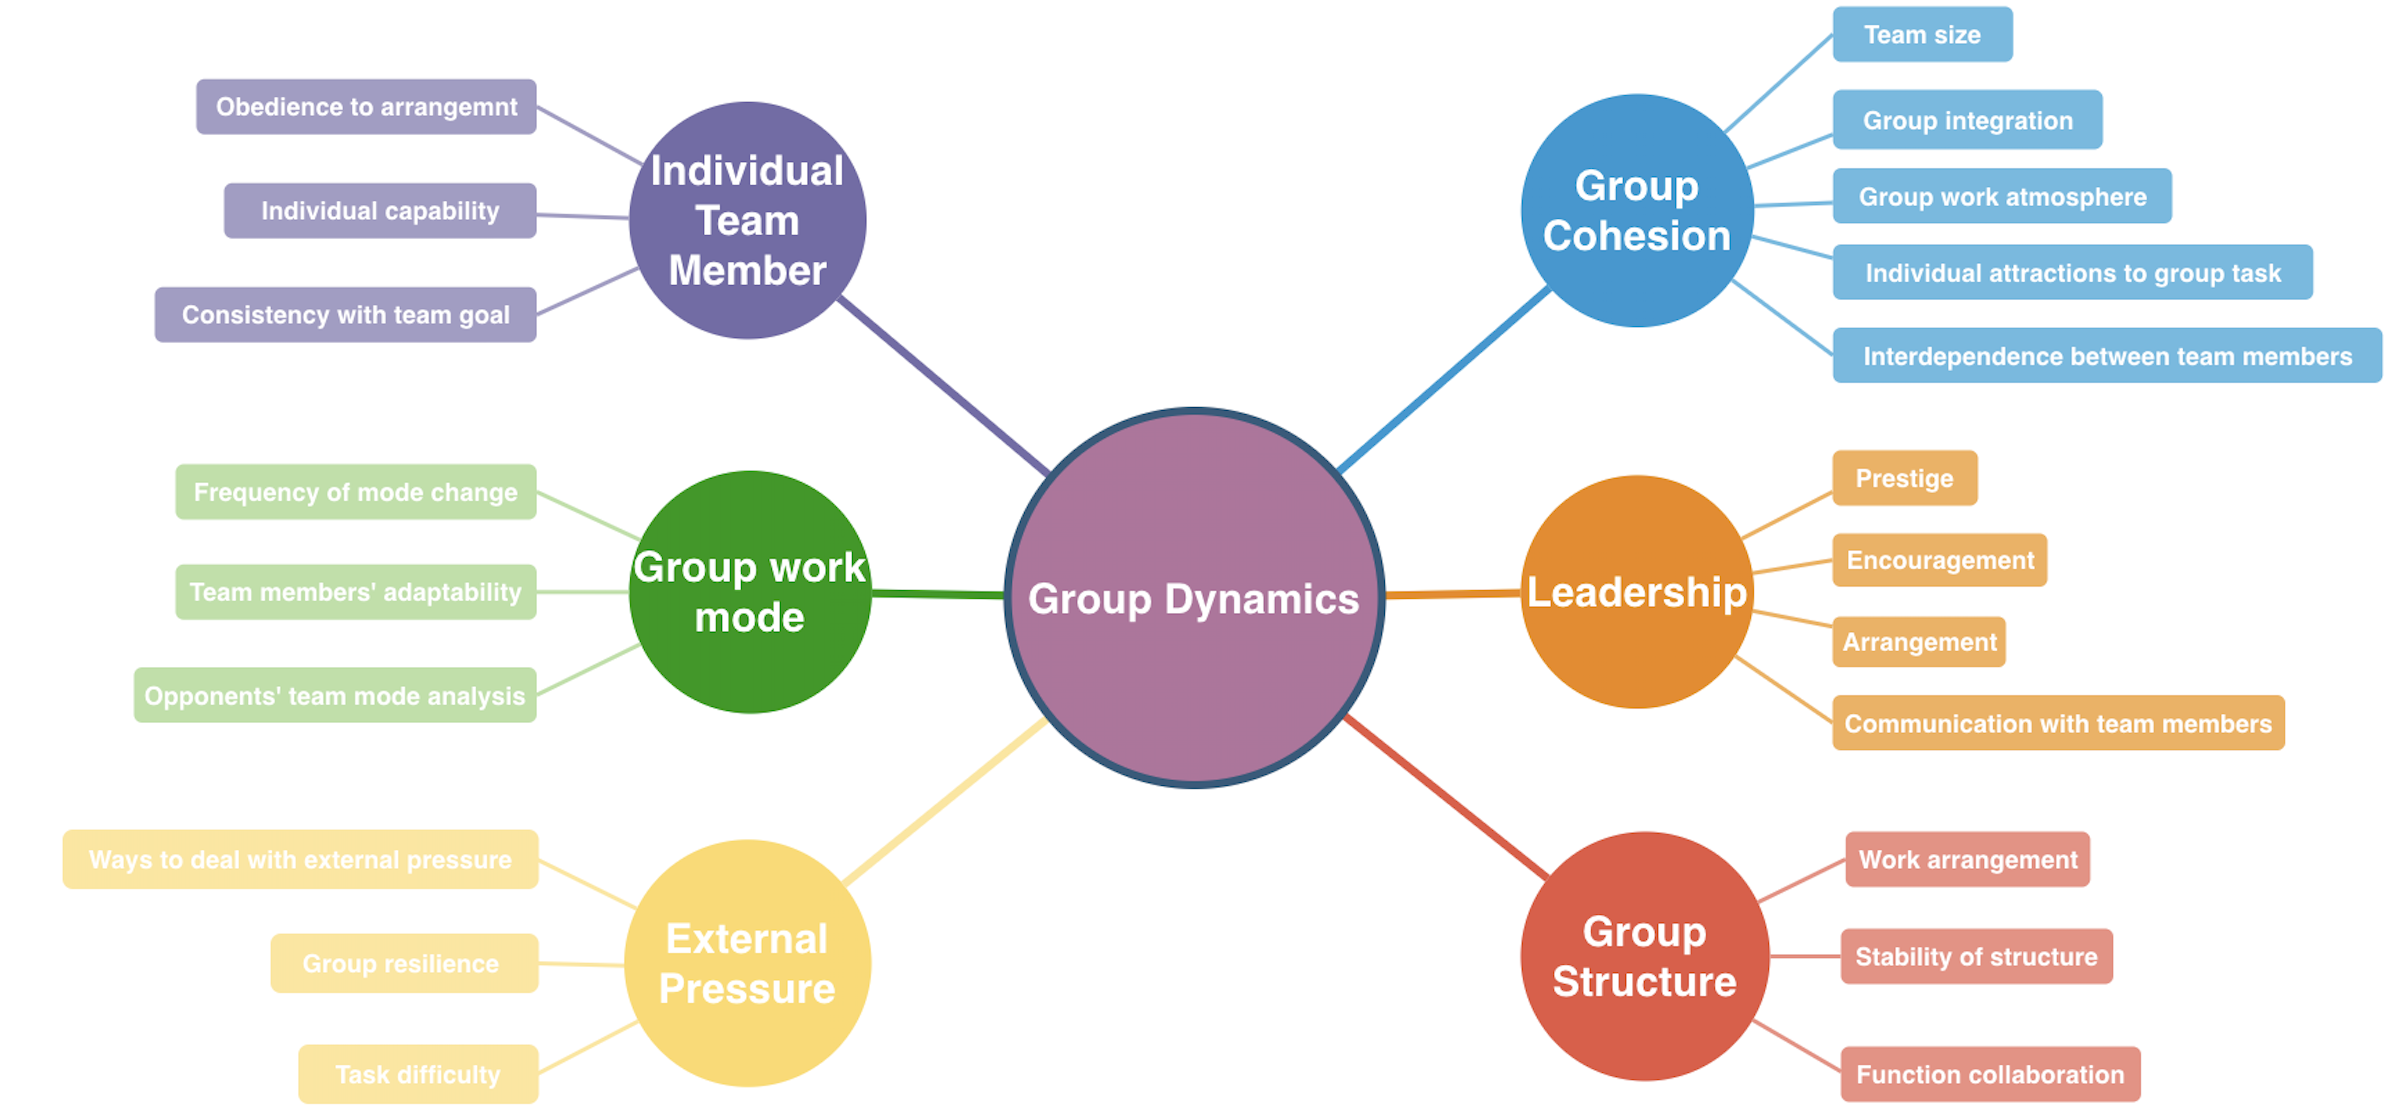
\includegraphics[scale=0.4]{images/mindmap.png}
    ~\\
    Figure 7. Mind Map of Group Dynamics.
\end{center}

\subsection{Implicational Generalizations in Team Design}
\subsubsection{Team Standard}

We should set criteria for selection of leaders and team members: In the case of clear team goals, it is necessary to formulate standards in order to select the appropriate team members and team leaders. This not only helps the formation of high-quality teams, but also updates the standards to give the members appropriate pressure and promote the continuous progress and development of team members . For instance, the marginal players in Huskies team will constantly strive to improve their strength to win more playing time and contribute more, and the core members will also keep fighting in order to maintain their core position. In this process, the overall strength of the team would be improved to a large degree
\subsubsection{Team Cohesion}
Team cohesion: a dynamic process that reflects the tendency of a group to remain united to pursue its instrumental goals and/or to meet the effective needs of its members\upcite{3}. Researches show that team cohesion has a positive relationship with the team's success in sports, and it is universal to social teamwork. Therefore, when designing an effective team, we need to ensure that this team has high team cohesion. This could be achieved by the following ways:
\begin{itemize}
    \item Increase the interdependence between team members: Huskies players work together, cooperate with each other, and give their peers full trust. In complex social teamwork, if team members are highly integrated with other members in behavior, emotion and psychology, it would easy to form a joint force, thus raising team cohesion; on the contrary, if the degree of interdependence in the achievement of goals is low, it would be hard to form team cohesion.
    \item Establish a team incentive model and promote a positive team atmosphere: under such model and atmosphere, team members can maintain their own good inner emotions, and at the same time, they can encourage other team members from different levels. The team ’s overall morale and confidence are strengthened to better complete tasks when members are supported by more psychological power.
    \item Form appropriate teamwork structure: When a team has a stable team structure, the cooperation between players will be more effective, and this dynamic balance can be maintained continuously. Therefore, in teamwork, appropriate and stable structures need to be designed for the responsibilities and arrangements of team members need to according to different settings, which can improve team cooperation, thus promoting the formation of stable team cohesion.
\end{itemize}
\subsubsection{Leadership}

In a football team, the coach and the team captain are the two leaders. The former trains the players, formulates the game strategy, field instructions and post-match summary; the latter's performance in the game will directly affect the team's performance. However, both of them need to establish prestige among team members, and play a role in encouraging morale and promoting team cohesion. From this point of view, the existence of leadership has great significance in social teamwork. In order to create a high-quality team, it is necessary to choose the right person for the leader, make them fully clear their responsibilities, mobilize the morale of the team, and direct the work of the leadership team.

\subsubsection{Individual Team Member}
\begin{itemize}
    \item Clarify the division of labor and responsibilities of each member: The goalkeeper, forward, midfielder and backcourt in Huskies have their most active areas and designated tasks. Only players in different positions play their strengths, complete their duties and actively cooperate with other members in the team can they score as many points as possible. Thus, under complex settings of teamwork, each member of the team needs to have a clear understanding of their own strengths and weaknesses, as well as other members of the team. On this basis, identify their main tasks and try their best to complete them.
    \item Obey instructions and arrangements: Players must obey the overall strategic arrangement of the coach during the game. They cannot completely go their own way and forget the team. Therefore, in teamwork, each team member must follow the overall arrangement of the team, and only the obedience of the team members can promote the orderly cooperation of a team.
\end{itemize}
\subsection{Additional Influencing Factors}

In order to to develop a more comprehensive generalized model of team performance, we also need detailed data on the following indicators, which might not be used in analyzing soccer game:
\begin{itemize}
    \item Team size: the size of the team is likely to affect the cohesion of the team under the different settings of team cooperation,  (the larger the team size, the less opportunities and possibilities for interaction between team members, which makes it difficult to form cohesion; on the contrary, if reducing team size, too much interaction may cause unnecessary contradictions and affect cohesion). Therefore, we need detailed data to analyze the impact of team size on team cohesion under specific settings.
    \item Task difficulty: the difficulty of a task directly affects team members' confidence and expectations for completing the task, and then affects team cohesion. By capturing the impact of task difficulty on team cohesion, we can consider adjusting the task difficulty in different ways in teamwork to improve the success rate of each task completion.
    \item Consistency of team members' goals: whether members within the team have consistent goals has an significant impact on achieving effective teamwork. Self-consciousness within the members will not only affect team cohesion, but also directly affect the team's ultimate success.
    \item External pressure level: threats from outside sources to force the team to accomplish the goal. Our preliminary assumption is that too high or too low external pressure is not conducive to promoting team vitality, so we need to find an appropriate level, and the definition of "appropriate" here depends on relevant index data.
\end{itemize}


\section{Strengths and Weaknesses}
    \subsection{Strengths}
        \begin{itemize}
            \item It is easy to visualize the performance in four aspects - attack, defense, collaboration and foul of one team in a match from our model.
            \item After evaluation, despite the small amount of data, the accuracy of our model is still relatively high.
            \item We did analysis on time-series activity data, which is an innovative idea.
            \item Fully utilize all aspects of data, for instance, our analysis covered both starting and alternate players
        \end{itemize}
    \subsection{Weaknesses}
        \begin{itemize}
            \item Possible to miss some detailed information hidden behind the frequency, such as some important events but happened only once.
            \item The current model is preliminary quantified, a larger size of data is needed for further improvement.
        \end{itemize}

\newpage
\begin{thebibliography}{99}
\bibitem{1} Buld\'{u}, J.M., Busquets, J., Echegoyen, I. et al. Defining a historic football team: Using Network Science to analyze Guardiola’s F.C. Barcelona. \textit{Sci Rep}, no. 9, (2019)
\bibitem{2}Cintia, P., Giannotti, F., Pappalardo, L., Pedreschi, D., \& Malvaldi, M. The harsh rule of the goals: Data-driven performance indicators for football teams.\textit{ 2015 IEEE International Conference on Data Science and Advanced Analytics (DSAA)}, (2015): 1-10.
\bibitem{3}Carron, A.V., Brawley, L.R. and Widmeyer, W.N. Measurement of cohesion in sport and exercise. \textit{In Advances in Sport and Exercise Psychology Measurement}, (1998): 213-226.
\bibitem{4}\url{https://graph-tool.skewed.de/static/doc/centrality.html}
\end{thebibliography}

\newpage
\begin{appendices}
		
\begin{verbatim}
    data.py
\end{verbatim}{}
\lstinputlisting[language=Python]{code/data.py}

\begin{verbatim}
    activity_level.py
\end{verbatim}{}
\lstinputlisting[language=Python]{code/activity_level.py}

\begin{verbatim}
    models.py
\end{verbatim}{}
\lstinputlisting[language=Python]{code/models.py}

\begin{verbatim}
    network.py
\end{verbatim}{}
\lstinputlisting[language=Python]{code/network.py}


        \begin{table}[h!]
			\centering
			\begin{tabular}{ccccc}
				\toprule
				& Attack & Defense & Collaborate & Foul \\
				\midrule
				Air duel  & 0.2 & 0 & 0 & 0\\
				Ground attacking duel  & 0.15 & 0 & 0 & 0\\
				Ground defending duel  & 0 & 0.15 & 0 & 0\\
				Ground loose ball duel  & 0.1 & 0 & 0 & 0\\
				Foul  & 0 & 0 & 0 & 0.1\\
				Hand foul  & 0 & 0 & 0 & 0.3\\
				Late card foul  & 0 & 0 & 0 & 0.1\\
				Out of game foul  & 0 & 0 & 0 & 0.3\\
				Protest  & 0 & 0 & 0 & 1.0\\
				Simulation  & 0 & 0 & 0 & 0.1\\
				Time lost foul  & 0 & 0 & 0 & 0.1\\
				Violent Foul  & 0.05 & 0 & 0 & 0.15\\
				Corner  & 0.1 & 0 & 0 & 0\\
				Free Kick  & 0.1 & 0 & 0 & 0\\
				Free kick cross  & 0.1 & 0 & 0.1 & 0\\
				Free kick shot  & 0.15 & 0 & 0 & 0\\
				Goal kick  & 0.2 & 0 & 0 & 0\\
				Penalty  & 0.1 & 0 & 0 & 0\\
				Throw in  & 0.2 & 0 & 0 & 0\\
				Goalkeeper leaving line  & 0 & 0 & 0 & 0.2\\
				Ball out of the field  & 0 & 0 & 0 & 0\\
				Whistle  & 0 & 0 & 0 & 0\\
				Acceleration  & 0 & 0 & 0 & 0\\
				Clearance  & 0 & 0.15 & 0 & 0\\
				Touch  & 0 & 0 & 0.15 & 0\\
				Cross  & 0 & 0 & 0.15 & 0\\
				Hand pass  & 0 & 0 & 0.1 & 0\\
				Head pass  & 0 & 0 & 0.15 & 0\\
				High pass  & 0 & 0 & 0.15 & 0\\
				Launch  & 0 & 0 & 0.1 & 0\\
				Simple pass  & 0 & 0 & 0.1 & 0\\
				Smart pass  & 0 & 0 & 0.2 & 0\\
				Reflexes  & 0 & 0.15 & 0 & 0\\
				Save attempt  & 0 & 0.1 & 0 & 0\\
				Shot  & 0.15 & 0 & 0 & 0\\
				Offside & 0 & 0 & 0 & 1 \\
				\bottomrule
			\end{tabular}
			\caption{Weights for different sub event type. }
		\end{table}	
		
	\end{appendices}
\end{document}




%% 
%% This work consists of these files mcmthesis.dtx,
%%                                   figures/ and
%%                                   code/,
%% and the derived files             mcmthesis.cls,
%%                                   mcmthesis-demo.tex,
%%                                   README,
%%                                   LICENSE,
%%                                   mcmthesis.pdf and
%%                                   mcmthesis-demo.pdf.
%%
%% End of file `mcmthesis-demo.tex'.
